\chapter{Introduction} % Main chapter title
%\selectlanguage{serbianc}
%\sffamily
%\fontencoding{OT2}\fontfamily{Tempora-TLF}\selectfont
%TODO: uvodni deo o prvom radu

Many real systems are composed of a large number of elements interacting with each other. Due to interactions, without any central force, the system exhibits the emergence of collective behaviour on the macro level\cite{kwapien2012}. Such a system is called a Complex System and its properties can not be predicted from the behaviour of the one individual \cite{ladyman2013}. An example of a complex system is the human brain. The structure of the brain network and its properties are fundamental for brain functioning, while an emergent phenomenon is a human intelligence. In societies, people's interactions lead to civilization, economy, formation of social groups. Also, the animal populations show different levels of organization that emerge from the individual's interactions \cite{boccaletti2006complex}. \cite{thurner2018} %latorro


The research in complex systems focuses on the structure of the interactions between units. Knowing how branches of the system are connected, we can determine the emergence of the collective behaviour of the system \cite{ladyman2013}. For the brain network, we can construct representation with neurons and synapses, representing the brain connectivity. Neurons in the same brain area are closely connected \cite{latora2017complex}. Similarly, we can define communication between people. The structure of these interactions gives us insights, for example, how information propagates through the system. The presence of people with many connections can lead to faster information flow. 

Despite the differences between complex systems, they can be studied using complex networks; with sets of nodes (vertices) and links (edges). Elements in the system are nodes, while interactions between them are given as edges. This approximation allows us to treat equally social \cite{myers2014, sarigol2014} (graph of actors) , biological (network of proteins) \cite{fraiman2009ising, schneider2011modeling} or even technological systems (internet, traffic) \cite{costa2007characterization, costa2011analyzing, newman2003structure}
%Analyzing and Modeling Real-World Phenomena with Complex Networks: A Survey of Applications
%Characterization of Complex Networks: A Survey of measurements

The complex network theory originates from the graph theory in mathematics. %These days, the graph and network are used as equivalent terms. 
The first mathematical problem solved using graph theory was $Konigsberg$ problem of seven bridges. The city $Konigsberg$ had seven bridges connecting the city's parts across the river and the island in the middle. The question was, is it possible to find a walk that crosses all seven bridges only once. Representing the problem as a graph, as in figure \ref{fig:Krgraph}, Euler managed to simplify the problem; the parts of the land are represented as nodes while bridges between them are links. Crossing each bridge only once is possible if each part of the land has an even number of connections. By this it is possible to enter one part of the land from one bridge and leave it by the other. As each node has odd number of connections, in this case it is not possible, see Fig. \ref{fig:Krgraph}.

\begin{figure}[!ht]
	\centering
	\includegraphics[width=0.3\linewidth]{Konigsberg_bridges.png} \hspace{2cm}
	\includegraphics[width=0.3\linewidth]{Konigsberg_graph.png}
	\caption{The Kronigsber problem of seven bridges.}
	\label{fig:Krgraph}
\end{figure}

The complex network theory is based on the graph theory and statistical physics are important for representation and description of the network structure. The complex network theory has application in different fields and the availability of the big data incurs its development. 

The analysis of different real networks showed that they share common properties \cite{boccaletti2006complex}: small-world behavior, large clustering and scale-free structure. Small-world property, means that distance between any two nodes is small and scales as logarithmic with the degree of the node. Real systems show high clustering, and most prominent feature is scale-free property, where the degree distribution follows power-law. 

The studies about dynamics of complex networks are necessary for understanding mechanisms which shape the structure of the real-world networks. Two decades before, mostly used complex network model was random network model (Erdős-Rényi), where each node has equal connecting probability, $p$ \cite{dorogovtsev2010complex}. This model produces Poisson degree distribution, contrary to the observed data so it could not describe real systems. Two seminal papers, from 1999., by Watts and Strogatz \cite{watts1998collective}, and Barabási-Albert model \cite{barabasi1999} inspired further research in this field. The Wattz and Strogatz  \cite{watts1998collective} proposed new model that could generate the networks with small-world propertites, while Barabasi-Albert model is able to generate the scale-free structures. The combination of network growth and linking rules- new nodes prefer high degree nodes- lead to scale-free degree distribution. Since then, different complex networks models were proposed in order to better describe the dynamics of social and technological systems. As linking probability in the B-A model is linear with node degree, first generalization was to introduce nonlinear dependence. Further, the linking probability may depend on the node age \cite{dorogovtsev2000b, dorogovtsev2001b}, or any other feature; fitness. Some models considered that nodes become inactive, or even that network grows through nonlinear number of links \cite{pham2016}. Models with accelerated growth \cite{sen2004} or in our paper we considered nonlinear growth in number of nodes. 

Important phenomena in statistical physics is called universality \cite{binney1992}. The empirical analysis showed that universality is characteeristic of many collective social phenomena  \cite{chatterjee2013, radicchi2008}. Even the growth of social groups, such as the growth of cities follow the universal patterns. The probability distribution of the cities sizes in one country follows same laws, with similar exponent for all countries \cite{barthelemy2019}. Understanding how universalities in the system emerge is also focus of statistical physics of complex systems \cite{verbavatz2020}. 

Beside empirical analysis and modeling complex networks, in order to characterize their strucure and dynamics, the important research direction is agent based modeling on the network topology.   

%TODO: uvodni deo o drugom radu
%TODO: uvodni deo o trecem radu

%In complex systems, the situation is even more difficult than in quantum mechanics, where there is uncertainty about the components, but not about its interactions. For many complex systems, not only can components be unpredictable, but the interactions between components can also become specific, time-dependent, non-linear, and unpre- dictable. However, there is still hope that probabilistic predictions about the dynamics and the collective properties of complex systems are possible. Progress in the science of complex systems will, however, be impossible without a detailed understanding of the dynamics of how elements specifically interact with each other. This is, of course, only possible with massive computational effort and comprehensive data.

%Physics largely follows an analytical paradigm. Knowledge of phenomena is expressed in analytical equations that allow us to make predictions. This is possible because interactions are homogeneous, isotropic, and of a single type. Interactions in physics
%typically do not change over time. They are usually given and fixed. The task is to work
%out specific solutions regarding the evolution of the system for a given set of initial and
%boundary conditions. 
%This is radically different for complex systems, where interactions themselves can
%change over time as a consequence of the dynamics of the system. In that sense, complex
%systems change their internal interaction structure as they evolve. Systems that change
%their internal structure dynamically can be viewed as machines that change their internal
%structure as they operate.

%Because of more specific and time-varying interactions and the increased variety of
%types of interaction, the variety of macroscopic states and systemic properties increases
%drastically in complex systems. This diversity increase of macrostates and phenomena
%emerges from the properties both of the system’s components and its interactions.
%The phenomenon of collective properties arising that are, a priori, unexpected from
%the elements alone is sometimes called emergence. This is mainly a consequence of the
%presence of generalized interactions. Systems with time-varying generalized interactions
%can exhibit an extremely rich phase structure and may be adaptive. Phases may co-exist
%in particular complex systems. The plurality of macrostates in a system leads to new types
%of questions that can be addressed, such as: what is the number of macrostates? What are
%their co-occurrence rates? What are the typical sequences of occurrence? What are the
%life-times of macrostates? What are the probabilities of transition between macrostates?
%As yet, there are no general answers to these questions, and they remain a challenge for
%the theory of complex systems. For many complex systems, the framework of physics is
%incomplete. Some of the missing concepts are those of non-equilibrium, evolution, and
%co-evolution. These concepts will be illustrated in the sections that follow.

%Scaling 

%Scaling laws of physics, however, are not the prime focus of this chapter. Here, we
%focus predominantly on scaling laws that appear in the statistical description of stochastic
%complex systems, where scaling appears in the distribution functions of observable quan-
%tities of dynamical systems or processes. The distribution functions exhibit power laws,
%approximate power laws, or fat-tailed distributions. In simple, non-complex statistical
%systems, such as gases, the underlying statistics is often the classical multinomial statistics
%that naturally leads to distribution functions that are either Gaussian or exponential. 1
%Many, if not most complex stochastic systems produce distribution functions that
%are fat-tailed or power laws. We discussed these in Section 2.4.1. Understanding their
%origin and how power law exponents can be related to the particular nature of a system,
%is one of the aims of the book. These questions will be discussed in some detail in
%Chapter 6. In this present chapter, we develop a feel for what scaling means in the
%context of complex stochastic systems and the forms it can take. We will define scaling


%TIme-series fractals (142 page)

%Understanding the interactions between the components of a system is key to under-
%standing it on a quantitative and predictive basis. In complex systems, interactions are
%usually not uniform, not isotropic, and not homogeneous: interactions between elements
%can be specific. Networks are a tool for keeping track of who is interacting with whom,
%at what strength, when, and in what way. Networks are essential for understanding
%co-evolution and phase diagrams of complex systems. Networks are also convenient for
%describing structures of objects, flows, and data. Practically everything that can be stored
%in a relational database is a network. Everything that can be related to, or associated with
%other things is part of a network. Mathematically, networks are matrices and, as such,
%are just a subset of linear algebra. Their importance and value for complex systems
%comes from their role in dynamical adaptive systems, where networks of interactions
%dynamically update the states of a system, and where the dynamics of states updates the
%interaction networks.

%Networks

%Complex systems are typically characterized by multiple types of interaction that occur between specific types of elements. For
%instance, interactions in social networks may consist of two individuals that exchange
%information by meeting each other either physically or through certain communication
%networks, such as mobile phones or online social networks. People without access to
%certain communication channels consequently cannot interact through that mode of
%communication. Networks serve as a book-keeping system to specify who interacts with
%whom, in what way, how strongly, when, and for how long.

%The field of network science in its modern form was triggered by two contributions
%in the late 1990s [28, 402]. As called for by Erdős and Rényi, these works defined
%classes of random networks that replaced the hypothesis of equal linking probability
%for all connections by more realistic assumptions. Watts and Strogatz were interested
%in the so-called small world puzzle, which is based on two seemingly contradictory
%empirical observations in many social, biological, and technological networks. On the
%one hand, certain networks are known to display high clustering and to consist of densely
%interconnected groups of nodes [339]. One would thus expect such networks to require a
%large number of steps to be ‘traversed’, as when a walker is on the network, he will more
%often than not get stuck in local clusters of nodes. On the other hand, however, such
%networks can, in reality, often be traversed in just a few steps. In social networks it has
%been shown with famous ‘letter passing experiments’ that the average ‘distance’ between
%any two individuals on the globe is about six [375]; hence the popular concept of ‘six
%degrees of separation’ [105, 401]. Watts and Strogatz reconciled these two observations
%by understanding ‘small world networks’: they showed that, starting from a network with
%very high clustering and very high distances, it only takes the addition of a relatively
%small number of random links (shortcuts) to create the small world effect. This idea had
%been anticipated by Mark Granovetter long before; he conjectured that social networks
%maintain cohesiveness on large scales due to so-called weak ties that act as bridges
%between well-connected groups of people [156].

%The second work that started the boom of network science was contributed by
%Barabási and Albert [28]. Their point of departure was the observation that many real
%world networks, such as the world wide web, have probability distributions of node
%degrees that follow power laws [8]. This means that there exist nodes that are extremely
%well linked—hubs. They introduced a simple model for the growth of networks to
%account for this observation: the Barabási–Albert (BA) model [28]. Starting from a small
%network with only a couple of nodes, new nodes that are preferentially linked to well-
%connected nodes are continually added to the network.

%If Erdős and Rényi had already anticipated these developments in 1960, why did it
%take more than thirty years to realize them? Naturally, the answer has to do with data
%availability and computer power [188]. In no other field are these developments as
%evident as in biology, which has essentially become a science of molecular and cellular
%networks [29, 200, 230]. Following the long tradition of networks in social science [398],
%economics [110, 190, 331], finance [5, 138, 165], and public health [75, 80] are now
%also starting to embrace networks. Network analysis has become one of the standard
%tools in data analytics [73, 291], along with regression models, time series analysis, and
%generative statistical models. Real networks are often much more heterogeneous than
%random networks such as those obtained from the ER or BA models. Links may be
%directed and undirected, spatially and temporally embedded, may only exist between
%different types of nodes that, in turn, may be related through links of more than one type;
%and all these properties are subject to constant dynamical changes and to the birth and
%death processes of nodes and links [54, 232]. Interest is currently shifting from simple
%and often static networks to generalized network structures that consist of multiple types
%of links and nodes—again, just as Erdős and Rényi predicted sixty years ago.

\selectlanguage{english}

\section{The complex networks}

The graph or network $G$ is defined as $G=(\boldsymbol{V}, \boldsymbol{E})$, where $\boldsymbol{V} = \{ v_1, v_2, ... v_N\}$ is a set of $N$ nodes (vertices), and  $\boldsymbol{E} = \{e_1, .. e_L\}$ is a set of $L$ edges (links). The edge is pair of nodes $e = (v_i, v_j), $ such that $\{v_i,v_j\}\in \boldsymbol{V}$. The most basic network representation considers \textbf{unweighted and undirected} structure. The edges are unweighted, meaning that all interactions in the network are equally important.  Because network is un-directed, edges are symmetric, such that $(v_i, v_j)$ implies $(v_j, v_i)$. In \textbf{directed} networks this simmetry is broken. The interaction between two nodes $v_i$ and $v_j$, can be only in one direction. A typical example is World Wide Web, where webpages are nodes and hyperlinks are directed edges. In biological networks, gene regulation and neural activation can be described as directed network. The first column a) in Figure \ref{fig:graph_dir} shows the graphical representation of two networks with equal number of nodes; the first one is underected and the second one is directed. 

Even though, graphical representation can be useful for describing the network structure, mathematical representation allow us to characterize the statistical properties of the networks. The graph $G$, with $N$ nodes could be represented with \textbf{adjacency matrix} $|A| = N \times N$ \cite{boccaletti2006complex}. The elements of the matrix are positive if there is connection between two nodes $v_i$ and $v_j$. 
\begin{equation}
A_{ij} =
\begin{cases}
1 & \text{ ($v_i$, $v_j$) $\in$ $E$}\\
0 & \text{ ($v_i$, $v_j$) $\notin$ $E$}
\end{cases}       
\end{equation}

The column b) on Figure \ref{fig:graph_dir} shows adjacancy matrix representation of given graphs. By convention diagonal elements $A_{ii}=0$, as self-loops are not allowed. For undirected network adjacency matrix is symmetric $A_{i,j}=A_{ji}$, but in the case of directed network matrix is not symmetric, as edges are drawn in one direction only.  

\begin{figure}[H]
	\centering
	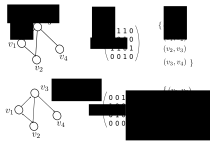
\includegraphics[width=0.7\linewidth]{directed_graph.pdf} 
	\caption{a) Graph representation of undirected (top panel) and directed (bottom panel) network. The same networks are represented with adjacency matrices column b), and edge list representation in column c).}
	\label{fig:graph_dir}
\end{figure}

The number of edges and nodes are dependent variables. Considering that each node can make $N-1$ connections, the maximum number of the edges in the network is $L_{max}=N(N-1)/2$, as each edge is counted twice. For directed network it is possible to draw $L_{max}=N(N-1)$ edges \cite{caldarelli2007scalefree}. When it comes to large networks, they are sparse, meaning that the number of links is $L<<L_{max}$. As consequence, the adjacency matrix is also sparse structure (has many zeros) that takes large portion of computer memory \cite{barabasi2016network}. 
It is common to represent the graph as edge list. In this case, illustrated on Figure \ref{fig:graph_dir}, column c), graph is described with the list of links that are in the graph, $G = \{ \{v_i,v_j\}\}$. Still with this representation we are not able to distinguish between directed and undirected graph structures, so in the computational algorithm should be specified if the edges are considered symetric or not.  


\begin{figure}[H]
	\centering
	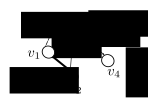
\includegraphics[width=0.4\linewidth]{multi_graph.pdf} 
	\caption{The complex networks may represent different characteristics of the system. The edges can be directed, weighted or multiply. Also nodes can be assigned with different weights or any relevant feature.}
	\label{fig:multigraph}
\end{figure}

To create the more realistic models, sometimes is essential to include the specific properties of the system in the network representation. For example, to emphasis the frequent interactions between nodes, edges can be assigned with different values, such networks are \textbf{weighted}. They can be described with adjacency matrix, whose elements can take any real number $A_{ij}=w_{ij}$ and $w_{ij}>0$. In general edges may be associated with any categorical variable. Similarly additional properties can be added to nodes, or even to the whole network structure. To include the \textbf{temporal} component in the network, edges are characterized with the time when the interaction between nodes happen. Finally, if two nodes interact in different ways, the \textbf{multigraph} is appropriate configuration where multiply edges are allowed. The graphical representation of discussed network representations is given on the Figure \ref{fig:multigraph}.

A \textbf{bipartite network} consists of two types nodes. The nodes in the same partition are not connected, while links exist only between partitions. For many real systems, a bipartite graph is a natural representation\cite{barabasi2016network, latora2017complex}. For example, the bipartite network of people and groups has two distinct node partitions while links indicate the memberships. Another example is a system of customers and products. The link between user and item is created when the user buys an item. The bipartite networks find their application in the algorithms for recommended systems, whose goal is to recommend items that may interest the user. Actually, to find the most probable missing links in the network. 

In a bipartite network, nodes in one partition are not connected. Still, we can analyse a single node type if we project the bipartite network on one partition. The primary assumption is that two nodes in one partition could be connected if they point to the same node in another partition. Consider the network of movies and actors. The one mode projection of movies is an undirected network whose links indicate that two movies share the same actors. On the other hand, another projection is a network of actors. The links exist if two actors appear in the same movie \cite{newman2010, barabasi2016network}.

\begin{figure}[H]
	\centering
	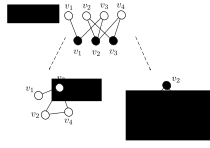
\includegraphics[width=0.7\linewidth]{bipartite_graph.pdf} 
	\caption{Bipartite graph and two partition projections.}
	\label{fig:gt2}
\end{figure}

We should be aware that important information is lost when creating a one-mode projection. First of all, without having weighted edges in the network of actors, it is impossible to have information on how many movies two actors appear in. From the one-mode projection, we can not reconstruct the original network. Moreover, two different bipartite networks may have the same projected networks. The important consequence of the network projection is the creation of cliques; subgraphs where all nodes are connected. \\
In general, it is possible to define the k-bipartite network. The same rules apply as before. There are $k$ distinct node partitions, while the edges exist only between different types of nodes.

\textbf{Temporal networks.}
Studying the real systems as static networks can give us a lot of insight into the system properties. Still, real systems are not static; they evolve not only in the number of elements but also in the number of interactions between them. Some interactions in the system may repeat in different intervals and could be described with complex activity patterns. Including time dimension in the network representation allows us to study the properties of the system closely. The temporal information may matter a lot \cite{holme2012}. For example if interaction between nodes $(v_1, v_2)$ happened before in time than  $(v_2, v_3)$, then nodes $v_1, v_3$ would not be connected, as it is the case in the static network. 

The temporal network is a collection of timestamped edges. Each edge is defined as $(v_i, v_j, t, \Delta t)$, where $v_i$ and $v_j$, are nodes $t$ is time when interaction happen, and $\Delta t$ is event duration \cite{guide_temporal}. The duration of the events may vary, as in the phone-call network. Also, for many systems, the time resolution of event duration is too small. For example, this parameter may be neglected when people interact on social platforms or email each other because the event time is too short, it scales in seconds.

\begin{figure}[H]
	\centering
	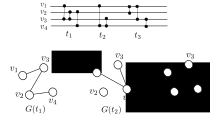
\includegraphics[width=0.7\linewidth]{temporal_network.pdf} 
	\caption{Temporal network. }
	\label{fig:gt3}
\end{figure}

The temporal network can be represented as sequence of static networks that evolve in time, $G = \{ G(t_1), G(t_2), ..., G(t_{max})\}$. At each time step, we can create the network and analyze the macroscopic properties of the given network snapshot. With this, we can end up with graph snapshots with many disconnected components or empty graphs for some points \cite{holme2015modern}. Sometimes, a much better approach is to aggregate the links that over time-windows. Here, we need to specify the time window length $w$. Interactions in the time interval $0\leq t<w$ enter the first snapshot. The next snapshot takes edges $w \leq t <2w$, and so on. The time windows are not overlapping, but generally, it is possible to slide the time window for different periods $ 1 \leq \delta t \geq w$. The downside of this method is that we can not recover original data points. The larger the time window is, the more information is lost. If the time window is set to $w=t_{max}$, there is only one snapshot, and the temporal data are no more available \cite{krings2012effects, arnold2021moving}. 

\textbf{Multilayer networks} were introduced for studying systems in which different types of interaction exist. This formalism allows one to investigate diverse network systems and to combine different types of data into one model \cite{porter2018multilayer}. In a multilayer or multiplex network, all nodes are present in each layer, but their interactions among layers differ. Two nodes may be connected in one layer but not in the other. Different online social systems may be an example of a multiplex network when users are connected on one platform but not on the other \cite{aleta2019multilayer}. Or the airline transportation network, where each layer represents the flights of different airline companies \cite{kivelamultilayer}.   

\newpage
\section{In this thesis}

In this thesis we use statistical physics and complex network approaches to model and empirically analyze online social systems. These systems consist of many users interacting in various ways on online platforms; the most natural underlying representation is the complex networks. In chapter \ref{Ch:Method}, we provide the methodology employed for this research. First, the theory of complex networks is discussed. Next, we describe the fundamental measures of complex networks and introduce basic complex network models. Section 2.5 reviews the most common probability distributions that characterize the properties of complex systems and outlines distributions fitting methods. Finally, we introduce the multifractality of the time-series and dynamical reputation model. 

The chapter \ref{Ch:signals} addresses the difference between network models where the growth in a number of nodes is constant and when it follows a non-trivial growth signal. This research aims to quantify how growth signals influence the structure of complex networks. Using the adapted ageing model \cite{hajra2004}, we use computer simulations to generate different kinds of complex networks. For more realistic real-world network simulations, growing signals are time series of new users from online social platforms, MySpace and Tech group from Meetup. They are described with trends, cycles and long-range correlations. Often time-series have multi fractal properties. The results of this study are published in \cite{vranic2021growth}, and they show the importance of growth signals in shaping the network structure because the scale-free networks, which represent real systems, are mainly altered. 

As research on social groups mainly focuses on a single group, there are remaining questions about the characteristics of the entire system. It has been shown that the distribution of company sizes follows log-normal behaviour and remains stable over decades \cite{stanley1996scaling}, and similar results are found for the sizes of cities \cite{barthelemy2016structure, barthelemy2019statistical}. For example, the Tech group is only one of the groups around which Meetup users organize; many other groups are created worldwide so system constantly grow. So far, there has been little research on the growth of online social groups. In chapter \ref{Ch:Groups} we will examine how groups on online social platforms grow. The results are summarized in the paper  \cite{vranic2022universal}. This research is based on the Reddit and Meetup data. From Meetup, we create two data sets, one with groups created in London and the other with groups created in New York, while for Reddit, we selected groups built before 2012. We are interested in explaining scaling behaviour in group size distribution and growth rates of group, identifying the growth mechanisms present in the system and providing the model that can reproduce the universality found in the system.

Even though across complex systems we find the emergence of universal behaviour, for example, the scaling of the degree distribution of two groups is similar, different factors might influence its success. It is well known that many online groups may suddenly fall apart. These questions are the subject of the chapter \ref{Ch:Trust}, which main results are published in the paper \cite{vranic2022sustainability}. Here, we study the question-answer platform Stack Exchange; it has more than 200 different topic-specified sites where people help each other in answering questions. What is interesting about this system is that some sites were closed because they did not produce enough activity. For that reason, we selected the sites with the same topic that failed but later, when someone proposed the site again, it stayed active. We analyze the evolution of user interaction networks and compare active and closed sites. We find that it is essential how the network users are distributed into a core-periphery structure \cite{gallagher2020clarified}. The core must selects firmly connected users, but their interaction with periphery has to be high. In other words, we need a trustworthy core to hold community. Introducing the Dynamical Reputation Model (DIBRM) \cite{melnikovDynamicInteractionBasedReputation2018}, based on user interaction sequences, we quantify how much users can be trusted and whether the community has a strong core. In the appendix \ref{App:SE} we briefly describe the Stack Exchange sites, in the appendix \ref{App:parameters} and \ref{App:sliding} discuss how we choose parameters  for DIBRM model while in appendix \ref{App:robust} we discuss the stability of inferred core-periphery structures. 

Finally, in the chapter \ref{Ch:Conclussion}, we draw the main findings of this thesis. 

\newpage










